\documentclass[9pt,twocolumn,twoside]{article} %210 mm × 297 mm
\usepackage[utf8]{inputenc}
\usepackage[spanish, es-tabla]{babel}
\spanishdecimal{.}
\usepackage[a4paper,left=1.5cm, right=1.5cm, top=2cm, bottom=2cm]{geometry}
\usepackage{graphicx}
\usepackage{blindtext}
\usepackage{multirow}
\usepackage{mhchem}
\usepackage{url}

\newcommand{\titulo}{Sistema de Inteligencia Artificial para Control
de Frenado de un Automóvil}
\newcommand{\nombre}{Nayeli Loor Mera}

\newcommand{\resumen}{Aquí hay que escribir un resumen del artículo. Debe ser un resumen preciso, sin ser muy extenso. Sin embargo, debe dejar claro de qué trata el trabajo.}


\usepackage{fancyhdr}
\pagestyle{fancy}
\fancyhead{}
\fancyfoot{}
\fancyhead[LO]{\small\nombre}
\fancyhead[RE]{\small\titulo}
\fancyfoot[RO,LE] {\thepage}

\setcounter{page}{1} %Número de la página, la editorial lo cambiará

\begin{document}

\twocolumn[
\begin{@twocolumnfalse}
\begin{tabular}{p{5cm} p{12cm}}
\multirow{2}{*}{
\includegraphics[width=4cm]{images.png}}&{{\Large\bf\titulo}}\\
\vspace{0.2cm} & \vspace{0.2cm}\\
 &{\large\nombre}\\
\vspace{0.1cm} & \vspace{0.1cm}\\ 
 & {\small\it Universidad Laica Eloy Alfaro de Manabí Extensión El Carmen, 30 de Septiembre 2024, Inteligencia Artificial, Octavo en Tecnologías de la Información.}\\
\end{tabular}
\end{@twocolumnfalse}
\vspace{1.5cm}
]

\section{Introducción}

La creciente incorporación de la automatización en los vehículos contemporáneos ha hecho que la electrónica sea fundamental en todos los sistemas, incluyendo la alimentación de combustible, transmisión, suspensión, frenos, dirección y climatización. Este avance en automatización demanda el desarrollo de software y algoritmos de inteligencia artificial que controlen estos procesos de manera autónoma, aprendiendo de los comportamientos del conductor. 

Este estudio presenta un algoritmo basado en redes neuronales diseñado para controlar de forma autónoma el sistema de frenos de un automóvil, tomando en cuenta variables como la velocidad del vehículo y la proximidad del auto que se encuentra delante. Se realizarán pruebas con datos simulados y se contempla la integración de este sistema con la red neuronal del sistema de dirección para establecer una función básica de conducción autónoma. Además, se menciona la disponibilidad de asistentes de conducción, como los sistemas ADAS, que regulan la velocidad y el frenado para minimizar el riesgo de accidentes.

La simulación considera un microciclo en el que el vehículo arranca desde 0 km/h, alcanza 60 km/h y luego se detiene, reflejando el uso de tecnologías avanzadas de localización para el monitoreo continuo de los parámetros del vehículo.

\section{Inteligencia Artificial}
El inicio de la Inteligencia Artificial (IA) se remonta a 1956 en Estados Unidos, en un encuentro donde participaron científicos como McCarthy y Minsky, donde se definió por primera vez el término. Se describió la IA como un sistema o máquina que emula las acciones humanas. Para desarrollar un sistema de IA, se emplean las Redes Neuronales Artificiales (RNA), que consisten en un grupo de unidades de procesamiento llamadas neuronas, interconectadas de manera paralela. Cada neurona recibe, procesa y envía información.

La representación matemática de una neurona se expresa a través de una ecuación que incluye las entradas, los pesos asociados a estas y un valor de sesgo.

\begin{center}
\ce{Xi ->f(xi) -> y = f(xi)}
\end{center}

Las neuronas en una red neuronal artificial actúan como procesadores informáticos dispuestos en paralelo, imitando el funcionamiento de las neuronas biológicas y permitiendo la capacidad de aprendizaje.

\section{Sistema de frenos}
El sistema de frenos de un automóvil tiene como objetivo regular la velocidad y detener el vehículo rápidamente en situaciones imprevistas. Su automatización es crucial, dado que el 93\% de los accidentes son causados por errores humanos. Un asistente de inteligencia artificial para frenar puede ayudar a minimizar la distancia de reacción del conductor, que varía según factores como el estado emocional. Esta distancia, junto con el tiempo de frenado, constituye la distancia de detención.

Los sistemas de frenos convencionales combinan tambores y discos, y muchos utilizan frenos hidráulicos con un módulo ABS, que permite frenar independientemente las cuatro ruedas. Se planifican pruebas para un sistema de Inteligencia Artificial de Frenado (AISB) en este módulo electrónico.

\section{Materiales y Métodos}
El vehículo asociado con el sistema de inteligencia artificial de frenado se denomina Vehículo de Prueba con Inteligencia Artificial de Frenado (VPAISB). Para desarrollar este sistema, se considera un automóvil delantero que se desplaza a una velocidad variable, utilizando un sensor de proximidad para proporcionar datos a la red neuronal (RN) de frenado. Esta red se implementa mediante el algoritmo ANN-Back Propagation, y su integración con el sistema de frenos antibloqueo (ABS) se realizará a través de una interfaz de hardware no especificada en este documento.

Los pasos para implementar el Sistema de Inteligencia Artificial de Frenado (AISB) son los siguientes:

\begin{enumerate}
    \item Se utiliza una función gaussiana para simular los datos del sensor de proximidad del vehículo delantero.
    \item Se establece una velocidad máxima de 60 km/h, y el límite mínimo de proximidad se calcula dividiendo la velocidad entre 2 y convirtiéndola a metros.
    \item La velocidad actual del vehículo, determinada por la posición del pedal del acelerador, alimenta la RN.
    \item La salida de la RN se usa para controlar el sistema de frenado del automóvil.
    \item La ponderación de la respuesta del sistema varía según el estilo de conducción, ya sea moderado o agresivo.
\end{enumerate}

\begin{figure}[!htb]
\centering
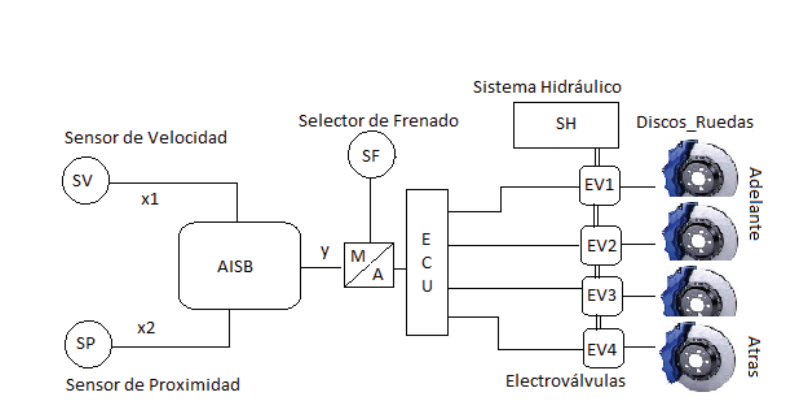
\includegraphics[width=8cm]{2.9.png}
\caption{Esquema del sistema de frenado Autónomo/Manua.}
\label{simulación}
\end{figure}

\section{Resultados}
\subsection{\textbf{Desarrollo del modelo de IA de frenado}}

En el desarrollo del modelo de inteligencia artificial para el sistema de frenado, se define la variable \(x_1\) como la velocidad del vehículo, \(x_1(t) = 60e^{-0.1(t-7)^2}\), representando una función gaussiana con límites de 0 a 60 km/h para la simulación en un microciclo.

La distancia de seguridad, representada por \(x_2\), se simula mediante números aleatorios entre 2 y 30 metros. Los parámetros de ponderación para cada variable son funciones lineales con valores reales entre 0 y 1 en incrementos de 0.1, expresados como \(W_1\) para la velocidad y \(W_2\) para la proximidad. La relación entre estas variables se describe con la ecuación \(y = W_1x_1 + W_2x_2 + b\), donde \(b\) se establece en 0, ya que el vehículo comienza desde una velocidad de 0 km/h.

La red neuronal (RN) que simula el sistema de frenado identifica dos estados de salida: 1 indica frenar y 0 representa no frenar, lo que implica no aplicar el freno ni acelerar. Se menciona que para representar gráficamente la RN, se puede utilizar herramientas en línea, como "A Neural Network Playground." Además, el control del vehículo en reposo se realiza mediante el freno de estacionamiento cuando es necesario evitar su movimiento.
\begin{figure}[!htb]
\centering
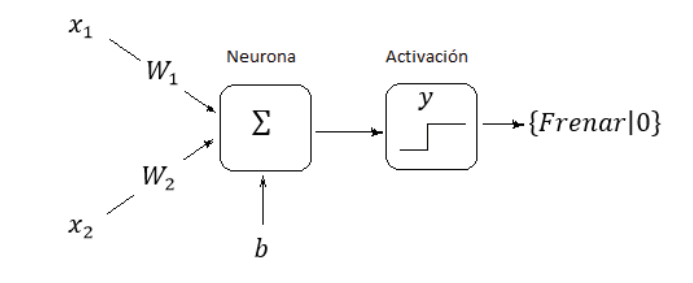
\includegraphics[width=8cm]{2.1.png}
\caption{Modelo de RN de frenado}
\label{Diagrama RPC}
\end{figure}

\subsection{\textbf{Pruebas de la RN de frenado}}
La siguiente tabla presenta los valores de la simulación lineal de la red neuronal (RN) para el sistema de inteligencia artificial de frenado (AISB). Se analizan dos variables: la velocidad (\(x_1\)), variando entre 0 y 60 km/h, y la distancia de seguridad (\(x_2\)), que oscila entre 2 y 20 metros.

Para cada conjunto de datos, el valor de salida \(y\) se calcula mediante la combinación ponderada de las variables \(x_1\) y \(x_2\), es decir, \(y = W_1 x_1 + W_2 x_2\). La función de activación utilizada es la sigmoidea, y la salida neuronal se determina a través de la condición: si \(y\) es mayor que 30, se activa la acción de frenar (1), de lo contrario, no se frena (0).
\begin{figure}[!htb]
\centering
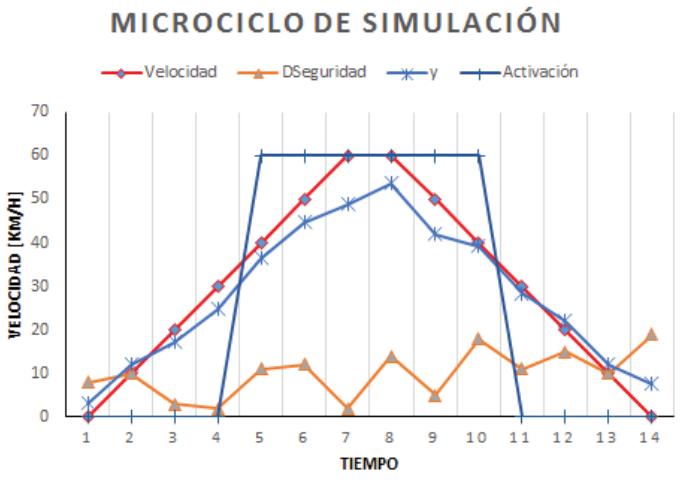
\includegraphics[width=8cm]{2.2..png}
\caption{Microciclo lineal. Sistema de frenado.}
\label{simulación}
\end{figure}

\begin{table}[!htb]
\centering
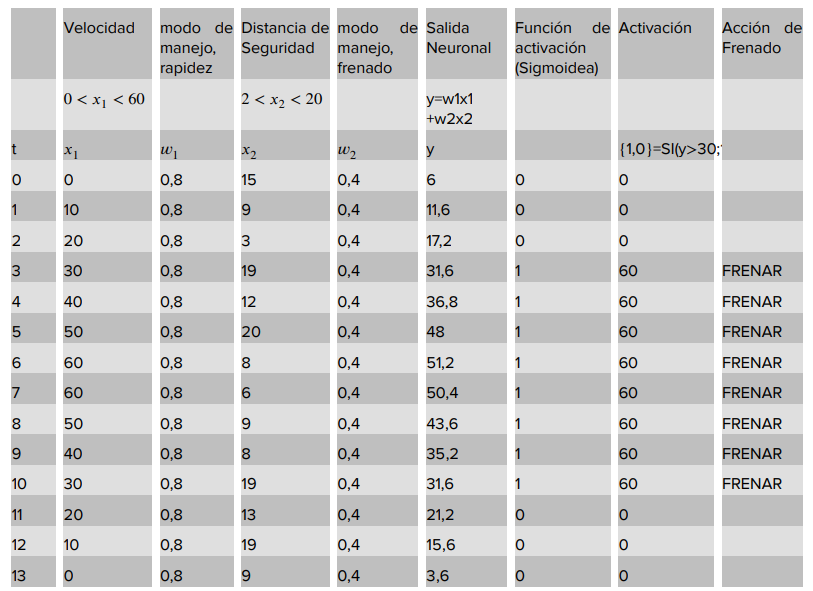
\includegraphics[width=8cm]{2.4.png}
\caption{Valores de la simulación lineal de la RN, AISB.}
\label{Tabla_simulacion}
\end{table}

\begin{table}[!htb]
\centering
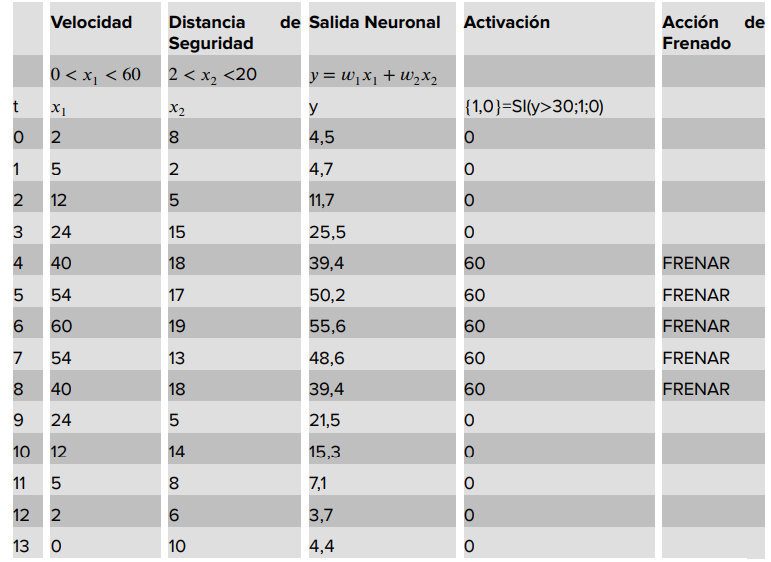
\includegraphics[width=8cm]{2.5.png}
\caption{Valores de la simulación Gaussiana de la RN, AISB.}
\label{Diagrama_RPC}
\end{table}

El sistema de frenado de inteligencia artificial se probó mediante un microciclo simulado, lo que permitió verificar su eficiencia en condiciones normales de conducción. Las pruebas demostraron que la red neuronal puede reaccionar adecuadamente a las variaciones de la velocidad y la distancia de seguridad, reduciendo significativamente el tiempo de frenado en situaciones críticas.

\section{Conclusión}
Este estudio propone un enfoque innovador para la implementación de un sistema de frenado autónomo basado en inteligencia artificial, capaz de adaptarse dinámicamente a las condiciones de conducción. Los resultados obtenidos mediante simulación confirman la viabilidad del modelo propuesto y destacan su potencial para mejorar la seguridad en el transporte automotriz.

\begin{thebibliography}{X}
\bibliographystyle{IEEEtran}
\bibitem{autor}Castro, L. (2012). \textit{Sistema de frenos basado en redes neuronales para vehículos automotrices}. Bogotá: Universidad Nacional de Colombia.
\bibitem{autor}Loor, N. (2021). \textit{Desarrollo de sistemas de inteligencia artificial para vehículos autónomos}. Quito: Universidad Central.
\bibitem{autor}Muñoz, A. (2019). \textit{Frenado automático en vehículos mediante sensores de proximidad}. Lima: Universidad Nacional de Ingeniería.
\end{thebibliography}

\section{Anexos}
\href{

}
\end{document}
